\chapter{Hiện thực và đánh giá}
\label{chap:experiment}

Trong thực nghiệm của đề tài với Gemini, union bốn arm phát hiện failure theo evaluator trên 92/1.454 PUT thuộc 36/157 task; Plain phát hiện 66 PUT. Pool nhiều arm sử dụng lượng dữ liệu và chi phí khác nhau. Kết quả dưới đây vì thế mô tả các detections bổ sung, chưa xác định hiệu quả khi cùng budget.

\section{Công nghệ và môi trường cài đặt}

Prototype được viết bằng Python, yêu cầu từ phiên bản 3.11. LangChain kết nối model; Pydantic kiểm tra schema; coverage.py đo thực thi; Hypothesis sinh dữ liệu trong arm có sampling. Các tests dùng pytest, còn Prefect quản lý cấu hình và trạng thái run. PUT chạy trong sandbox trên Linux. Các công cụ này được giới thiệu ở Mục~\ref{sec:related-technologies}.

Manifest của run Gemini ghi Python 3.11.14, coverage 7.17.0, Pydantic 2.14.2, Hypothesis 6.170.14, python-graphs 1.2.3, EvalPlus 0.3.1 và langchain-google-vertexai 3.2.5. Đây là phiên bản thực tế của snapshot thí nghiệm. Thực nghiệm chưa tổng hợp đủ thông tin CPU, RAM và thiết bị phục vụ inference để so sánh thời gian xử lý giữa các môi trường; latency và throughput chưa được đánh giá.

\section{Phần công việc thực hiện và phần kế thừa}

Phần cài đặt ở cấp đề tài gồm adapter đưa các arm về hợp đồng input chung, CallBuilder gắn dữ liệu theo chữ ký, context và stage interfaces, freeze/manifest checks, bộ tổng hợp detections theo arm và các regression tests. Các phần này cho phép thay cách sinh dữ liệu trong khi giữ chung reference và scorer. Runtime, checkpoint, bộ đo và adapter model được tích hợp để lưu bằng chứng của từng lần thực thi.

Phần kế thừa gồm các kỹ thuật kiểm thử kinh điển, đặc tả HumanEval, references từ HumanEval+, mô hình đã huấn luyện và thư viện bên thứ ba~\cite{chen2021evaluating,liu2023evalplus}. Công việc cài đặt cần phân biệt phần sử dụng lại với phần tích hợp và phép kiểm tra do đề tài xây dựng.
Việc chia module trong Chương~\ref{chap:method} mô tả sản phẩm tích hợp của đề tài. Phân công cài đặt cá nhân cần được sinh viên xác nhận trước khi ký bản nộp; danh sách module không thay thế xác nhận đó.

\section{Câu hỏi và thiết lập đánh giá}

Thực nghiệm xem xét arm nào tạo detection ngoài Plain, union bổ sung bao nhiêu PUT và coverage C1/C2 thay đổi ra sao.

\subsection{Dữ liệu, đối sánh và budget}
\label{sec:experiment-data}

Run sử dụng 164 task slots, trong đó có 157 task đủ điều kiện với 1.454 base-pass PUT. Năm task không có base-pass PUT là 65, 127, 132, 145 và 163; hai task thiếu số cài đặt theo cohort là 32 và 136. Bảy skips này được quyết định từ cohort trước sinh input. Run không có generation failures hoặc evaluation failures. Đặc tả lấy từ HumanEval và references lấy từ HumanEval+~\cite{chen2021evaluating,liu2023evalplus}. Đề tài cố định bản reference v0.1.10, chỉ giữ mã tham chiếu và metadata; không đưa hidden test inputs vào bản xuất này.

Số liệu trong chương là kết quả thực nghiệm của đề tài ngày 12/11/2026. Các bảng detection được đối chiếu với kết quả từng task và hai tệp \path{result_digest.json}, \path{union_result.json} của run.\footnote{Mã run: \path{4e3a4d78-1a06-4b07-93cf-7054a0ec1a6c}; thư mục dữ liệu: \path{final/out/gemini_full4_20261112_074012/}.} Đây là dữ liệu thực nghiệm do đề tài tạo ra, được ghi riêng với các tài liệu tham khảo bên ngoài.

Model là \texttt{gemini-3.1-flash-lite} qua Vertex AI. Mỗi arm có budget tối đa 20 input/task; completion cap là 4.096 tokens/call, context cap là 18.192 tokens và native timeout là 8 giây. Plain, EP+BVA v2 và DT v2 tối đa một completion/task, còn Control-flow tối đa hai vòng/task. Control-flow sử dụng cả Hypothesis sampling.

Toàn run có giới hạn 785 logical calls và 2.355 transport attempts. Thực tế nhận được 629 responses trong 630 attempt records, với một unknown attempt. Phần usage đã biết gồm 1.858.543 prompt tokens và 363.459 completion tokens, tổng cộng 2.222.002 tokens; chưa có usage của unknown attempt.

Plain sinh input trực tiếp. EP+BVA v2 và DT v2 dùng hướng dẫn theo kỹ thuật tương ứng; Control-flow dùng thông tin cấu trúc và công cụ hỗ trợ. Tên arm chỉ cấu hình sinh dữ liệu. Việc dữ liệu thực hiện đúng các lớp, biên hoặc rule còn cần phép kiểm tra ngữ nghĩa riêng.

\subsection{Các đại lượng đánh giá}

Detected PUT là cài đặt có ít nhất một input thuộc arm tạo failure được evaluator xác nhận theo protocol của run. Mỗi PUT được đếm một lần trong một arm hoặc pool. Task có detection là bài toán có ít nhất một PUT như vậy. Valid inputs đếm input memberships được chấp nhận cho từng arm; khi hợp các arm, input trùng phải được dedup.

Với tập detections $D_A$ của arm $A$ và tập $D_P$ của Plain, số detection ngoài Plain là $|D_A\setminus D_P|$. Số này khác chênh lệch $|D_A|-|D_P|$ vì hai tập có thể chứa các PUT khác nhau. Union được tính bằng hợp tập có dedup theo danh tính PUT, không cộng trực tiếp raw counts.

Failure được chia thành wrong-value, exception và resource. Resource gồm timeout, RecursionError và MemoryError. Nếu một PUT có nhiều loại failure, phép tổng hợp ưu tiên wrong-value, rồi exception, cuối cùng resource để đếm PUT vào đúng một nhóm.

\section{Kịch bản kiểm thử prototype}

Bảng~\ref{tab:prototype-tests} mô tả các trường hợp kiểm tra hợp đồng của prototype. Các trường hợp này kiểm tra cách xử lý dữ liệu và lỗi trong công cụ. Kết quả benchmark được trình bày từ Mục~\ref{sec:detection-results}.

\begin{table}[htbp]
\centering
\caption{Các kịch bản kiểm thử hợp đồng của prototype}
\label{tab:prototype-tests}
\small
\begin{tabular}{p{0.08\textwidth}p{0.34\textwidth}p{0.45\textwidth}}
\toprule
Mã & Tình huống kiểm tra & Kết quả mong đợi \\
\midrule
TC01 & Một biến tháng, normal BVA & Nhận đủ 1, 2, nominal, 11, 12 và thiết kế 5 ca \\
TC02 & Hai chiều, single-fault & Đo thiết kế 9 ca; không tính đổi đồng thời hai chiều như ca single-fault \\
TC03 & Hai lớp EP chồng lấn & Báo overlap trong cùng trục phân hoạch \\
TC04 & Rule DT sau gộp & Không tăng giả độ phủ trên các original rules \\
TC05 & Robust BVA thiếu đặc tả ngoài miền & Báo không áp dụng trước model call \\
TC06 & Catalogue sai, input vẫn hợp lệ & Giữ input cho đánh giá và ghi lỗi catalogue riêng \\
TC07 & Reference được yêu cầu trước input freeze & Từ chối để bảo vệ hợp đồng đánh giá \\
TC08 & Replay thiếu manifest hoặc có live calls & Từ chối; không tự tạo workload bù \\
TC09 & Dữ liệu/setting thay đổi so với manifest & Phát hiện sai khác trước generation \\
TC10 & Số kết quả evaluation thiếu input & Báo lỗi; không bỏ im lặng các input chưa có kết quả \\
TC11 & Sandbox truy cập host hoặc credentials & Không nhìn thấy tài nguyên ngoài policy \\
TC12 & Chương trình lặp vô hạn & Kết thúc theo timeout thay vì treo toàn run \\
\bottomrule
\end{tabular}
\end{table}

TC01--TC06 kiểm tra các fixtures EP/BVA/DT và integration tests. TC07--TC09 kiểm tra pipeline và replay; TC10 kiểm tra số lượng kết quả evaluation; TC11--TC12 kiểm tra giới hạn runtime. Lần kiểm tra phục vụ hoàn thiện bản thảo chạy năm test modules tương ứng, ghi nhận \textbf{69 tests pass trong 15,87 giây}, không có failure hoặc skip. Số test lớn hơn số kịch bản vì một kịch bản có thể gồm nhiều giá trị tham số và test modules còn chứa các regression cases liên quan.

Kết quả này được đọc từ output pytest mới, không dẫn lại một report tổng hợp trong repository. Các tests dùng fixtures và sandbox local; không gọi model hay chạy benchmark HumanEval mới. Phạm vi kiểm tra gồm hợp đồng dữ liệu và runtime đã chọn, không phải toàn bộ working tree hoặc mọi nhánh Control-flow. Lệnh tái lập và mapping nằm trong Phụ lục~\ref{app:reproduction}.

\section{Trình diễn từ run đã hoàn tất}
\label{sec:demo}

\subsection{Xem hồ sơ run và artifact}

Demo sử dụng run Gemini đã hoàn tất, không yêu cầu inference lại. Người xem mở trang Runs của Prefect, chọn run có ID đã nêu ở Mục~\ref{sec:experiment-data}, kiểm tra trạng thái và mở artifacts chứa config, tiến độ và kết quả. Config xác nhận model cùng budget; kết quả cho biết 164 slots đã xử lý, gồm 157 task evaluation và 7 skips. Một hồ sơ Completed cần được đọc cùng các con số này để biết phạm vi thực sự hoàn tất.

Hình~\ref{fig:prefect-demo} là ảnh giao diện thật khi mở record này. Gemini chạy bằng external runner rồi được observer ghi vào Prefect, nên vùng task/subflow graph có thể trống. Các bước trong Hình~\ref{fig:task-flow} là luồng xử lý của chương trình, không phải task DAG đã đăng ký với Prefect.

\begin{figure}[htbp]
\centering
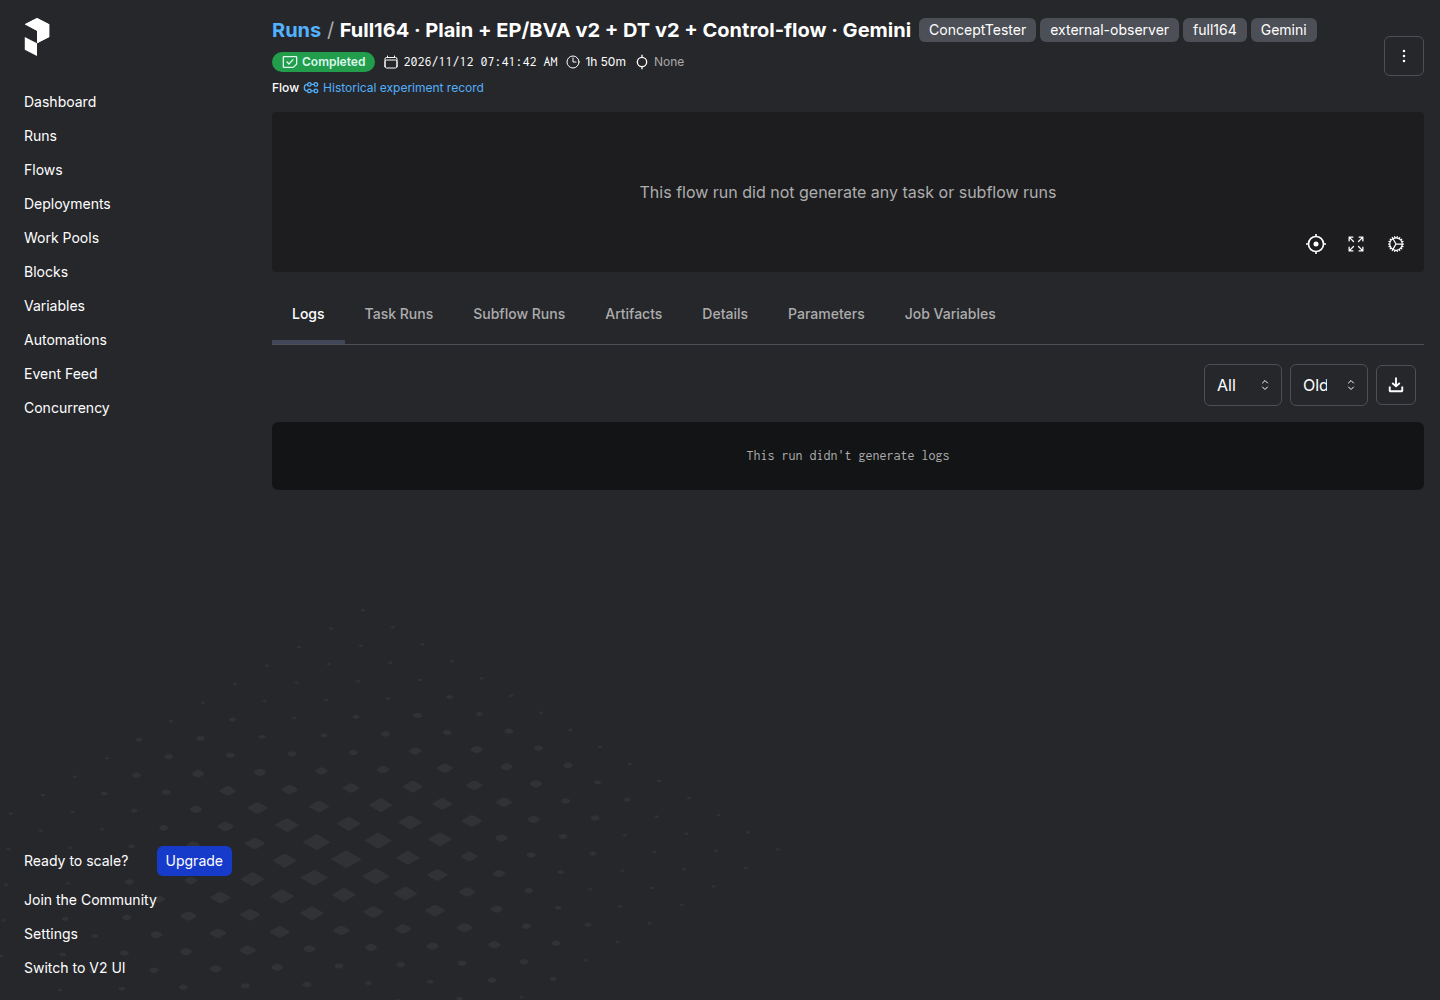
\includegraphics[width=\textwidth]{figures/prefect-run.png}
\caption[Record thực nghiệm Gemini trên Prefect]{Record thực nghiệm Gemini Completed trên Prefect local. Ảnh chụp trực tiếp trong lần hoàn thiện bản thảo, không khởi chạy run mới.}
\label{fig:prefect-demo}
\end{figure}

Từ một task result, người xem chọn arm và PUT ID, lấy failing index rồi tìm input tương ứng trong oracle tests. Hai evaluation checkpoints cho biết status và actual ở lượt đầu và lượt xác nhận. Đây là đường truy nguyên một detection; đọc summary riêng lẻ không cho biết input nào tạo ra sai khác.

\subsection{Ví dụ có detection bổ sung: kiểm tra định dạng ngày}

Trong task HumanEval/124, đặc tả yêu cầu chuỗi dạng \texttt{mm-dd-yyyy} và cho phép tháng 2 có ngày từ 1 đến 29. Đặc tả này không yêu cầu xét năm nhuận. DT v2 sinh input \texttt{02-29-2001}; reference trả \texttt{True}, trong khi PUT 7 trả \texttt{False} ở cả hai observations. PUT dùng \texttt{calendar.monthrange}, nên loại ngày 29 tháng 2 của năm 2001 theo lịch thực tế và trái quy tắc riêng của task.

Input nằm ở index 26 trong union tests của task. Failing indices của PUT 7 và retested indices cùng chứa 26, hai checkpoints đều ghi \texttt{fail}. Plain, EP+BVA v2 và Control-flow không có detection PUT 7 trên inputs của chúng trong run này. DT v2 vì vậy có một detection bổ sung so với ba nguồn đó trên task 124.

Catalogue của DT v2 ở task này có status \texttt{catalogue\_invalid}, nhưng 16 inputs vẫn qua reference và được chấm. Ví dụ minh họa vì sao decoder giữ input hợp lệ khi metadata concept lỗi. Detection xác nhận một sai khác theo spec của task; nó chưa chứng minh rule catalogue hoặc mọi Fault Hypothesis của model đúng ngữ nghĩa.

\subsection{Ví dụ target không đồng nghĩa với bug}

Ở HumanEval/0, Control-flow đề xuất concept \texttt{single\_element\_list}, với quan hệ \texttt{len(numbers)==1} và một target C2 có owner PUT cụ thể. Strategy giới hạn danh sách một phần tử, còn \texttt{threshold} nhận 0,5. Model cũng đề xuất danh sách rỗng cho nhánh liên quan. Arm kết thúc với năm selected inputs qua reference, nhưng không phát hiện PUT nào của task này.

Ở task 125, Control-flow tiếp tục tạo các chuỗi có comma và không chứa literal space để thử một nhánh. Cả bốn arm đều có 20 valid inputs và đều không có detection trên task đó trong run Gemini. Đây là kết quả của run đang mô tả; không thay bằng witness từ một run Qwen khác để làm ví dụ thành công. Target, input hợp lệ và failure là ba mốc cần ghi nhận riêng.

\section{Kết quả phát hiện theo evaluator}
\label{sec:detection-results}

Bảng~\ref{tab:gemini-arms} trình bày kết quả từng arm trong run ở Mục~\ref{sec:experiment-data}. Mẫu số là 1.454 PUT và 157 task đủ điều kiện.

\begin{table}[htbp]
\centering
\caption{Kết quả từng arm trong run Gemini đã lưu}
\label{tab:gemini-arms}
\begin{tabular}{lrrr}
\toprule
Arm & Valid inputs & Detected PUT/1.454 & Task/157 \\
\midrule
Plain & 2.231 & 66 & 26 \\
EP+BVA v2 & 1.556 & 68 & 28 \\
DT v2 & 1.640 & 72 & 28 \\
Control-flow & 732 & 35 & 11 \\
\bottomrule
\end{tabular}
\end{table}

DT v2 có nhiều detections nhất trong run này. Các arm cùng input cap nhưng số input hợp lệ khác nhau, như Bảng~\ref{tab:gemini-arms} cho thấy. Xét những PUT chưa được Plain phát hiện, EP+BVA v2 bổ sung 17, DT v2 bổ sung 21 và Control-flow bổ sung 2.

Bảng~\ref{tab:gemini-unions} hợp các detections đã xác nhận ở từng task. Mỗi PUT chỉ được đếm một lần trong một pool.

\begin{table}[htbp]
\centering
\caption{Detection trên một số union đầu vào Gemini}
\label{tab:gemini-unions}
\small
\begin{tabular}{p{0.38\textwidth}rrrr}
\toprule
Pool & Wrong-value & Exception & Resource & Tổng PUT \\
\midrule
Plain & 60 & 1 & 5 & 66 \\
Plain + EP+BVA v2 & 72 & 5 & 6 & 83 \\
Plain + DT v2 & 76 & 3 & 8 & 87 \\
Plain + Control-flow & 61 & 1 & 6 & 68 \\
EP+BVA v2 + DT v2 & 66 & 5 & 8 & 79 \\
Plain + EP+BVA v2 + DT v2 & 78 & 5 & 9 & 92 \\
Cả bốn arm & 78 & 5 & 9 & 92 \\
\bottomrule
\end{tabular}
\end{table}

Union bốn arm bổ sung 26 PUT ngoài Plain, gồm 18 wrong-value, 4 exception và 4 resource. Union Plain, EP+BVA v2 và DT v2 đã đạt 92 PUT. Cả 35 detections của Control-flow đều nằm trong tập của EP+BVA v2 và trong tập của DT v2, nên thêm Control-flow vào pool ba arm không tăng detection ở run này.

\section{Kết quả bao phủ C1/C2}

Phép đo coverage chạy base tests cùng union accepted inputs của bốn arm trên toàn bộ source, gồm các hàm hỗ trợ. C1 được đo bằng executable source lines, C2 bằng branch arcs của coverage.py. Bộ đo thực hiện 11.379 input traces trên 1.454 PUT với timeout 1 giây/input; có 10 PUT ghi nhận timeout và không có trace errors.\footnote{Mã run coverage: \path{0b1828c7-a222-4a07-a431-2d712a3149c5}. Kết quả từng PUT và tệp \path{result_digest.json} nằm trong \path{final/out/gemini_full4_coverage_20261112/}.}

Bảng~\ref{tab:gemini-coverage} đếm số PUT đạt 100\% theo từng tiêu chí; bảng không tính coverage trung bình của cohort.

\begin{table}[htbp]
\centering
\caption{Số PUT đạt 100\% coverage trước và sau khi thêm union inputs}
\label{tab:gemini-coverage}
\small
\begin{tabular}{p{0.43\textwidth}rrr}
\toprule
Tiêu chí & Mẫu số PUT & Base & Base + union \\
\midrule
C1: executable lines & 1.454 & 1.050 & 1.193 \\
C2: PUT có branch & 1.151 & 697 & 865 \\
Cả C1/C2, gồm 303 PUT không branch & 1.454 & 992 & 1.148 \\
\bottomrule
\end{tabular}
\end{table}

Base cộng union tăng 143 PUT đạt toàn bộ executable lines và 168 PUT có branch đạt toàn bộ branch arcs. Trong hàng cuối, 303 PUT không branch được xem là không có nghĩa vụ C2, nhưng vẫn phải đạt đủ C1. Phép đo dùng cả base và generated inputs, chỉ xét C1/C2. Với trace timeout, coverage dưới 100\% có thể là lower bound; phép đo này cũng chưa kiểm tra lại toàn bộ base contracts của baseline.

\section{Thảo luận và giới hạn kết luận}

EP+BVA v2 có 68 detections so với 66 của Plain, nhưng bổ sung được 17 PUT ngoài Plain. Chênh lệch tổng số chỉ là 2 vì hai arm bỏ sót những PUT khác nhau. Khi quyết định có thêm một arm vào pool hay không, cần xét phần detection riêng này cùng chi phí tăng thêm.

Oracle có thể đánh giá sai ở bài toán có nhiều đáp án hợp lệ. Số input hợp lệ, số rounds và sự tham gia của sampler cũng khác nhau giữa các arm. Chưa có ablation tách đóng góp concept khỏi các yếu tố này. Tập thí nghiệm chưa có ground truth đầy đủ để tính precision, recall hoặc accuracy.

Kết quả áp dụng cho cohort và model đã công bố. Các run Qwen hoặc protocol có timeout khác cần được phân tích riêng trước khi so sánh. Thực nghiệm này chưa chuẩn hóa phép đo latency, throughput hoặc chi phí tiền.
